\subsection{number equation}
Put \eef{eq:20100915:F} into number equation \eef{eq:20100909:number}, we have\footnote{Here we drop $\sgn_{k}$ as $(\epsilon^{ab}_{\vk}-2\mu+  G_{0}^2\eta)$ takes care of the sign}
\begin{equation}\label{eq:20101011:number}
N=\sum{1-\sqrt{1-4G_{k}^{2}}\frac{(\epsilon^{ab}_{\vk}-2\mu+  G_{\vk}^2\eta)}{{\sqrt{{(\epsilon^{ab}_{\vk}-2\mu+  G_{\vk}^2\eta)^{2}+\Delta^{2}}}}}}
\end{equation}
This equation also requires to take into account that $G_{k}$ approaches 0 at high momentum to be convergent.  
\subsection{typical energy scale}
I calculated $^{6}\text{Li}$'s Fermi energy for density $10^{15}\text{cm}^{-3}$, it is $5\times10^{-28}J$, for Bohr magneton $\mu_{B}=9.27\times10^{-24}\text{J T}^{-1}$, it corresponds magnetic field $B=0.5\times10^{-4}\text{T}=0.5\text{G}$. On temperature side, it is about $3\times10^{-5}\text{K}$ with ($k_B=1.38\times 10^{-23}\text{J K}^{-1}$). 

On the other hand
\[
 \frac{\hbar^2}{m_{\text{Li}}a_0^2}\approx10^{-24}\text{J}\sim0.1\text{K}
\]


\subsection{more on $G_{k}$ and $\eta$}
$\phi^{0}$ the w.f. of two-body close-channel bound state varies in different Feshbach resonance and is a case-specific quantity.  Its relevant property is included in the general two-body Feshbach resonance formula's $\Delta{B}$.  However, its other properties does matter in narrow resonance problem.  Fortunately, this can be simplified if it is a close-to-threshold bound-state, that mostly is outside the potential.  Therefore, most weight of $\phi^{0}$ follows the simple form 
\[
\phi^{0}(r)=C\frac{e^{-\kappa{r}}}{r}
\]
 where $\frac{\hbar^{2}\kappa^{2}}{2m}=E^{0}$ and $\kappa>0$.  $C^{2}=\frac{\kappa}{2\pi}$.  Convert it into k-space
 \begin{equation}\label{eq:20101011:phi}
\phi^{0}_k=\nth{(2\pi)^{\frac32}}\int{d^{3}\vr\phi^{0}(r)e^{-i\vk\cdot\vr}}=\nth{\pi}\frac{\kappa}{k^{2}+\kappa^{2}}
\end{equation}
Now we can estimated $G_{k}^{2}\eta$. $G_{k}=\alpha\phi^{0}_{k}$ where 
\[|\alpha|^{2}<n\sim{E_{F}^{3/2}}\]
\[
\abs{\phi^{0}_{k=0}}^{2}=\nth{\pi^{2}\kappa^{3}}\sim\nth{(E^{0})^{3/2}}
\]
And $\eta\sim{E^{0}}$, So 
\[
G_{k}^{2}\eta<G_{k=0}^{2}\eta<E_{F}(\frac{E_{F}}{E^{0}})^{1/2}
\]
And we have $E_{F}\ll{E^{0}}$, so this term is much smaller than $\mu\sim{E_{F}}$ in BCS side. For now, we just omit this term.  Considering $G_{k}^{2}\ll1$, we can expand $\sqrt{1-4G_{k}^{2}}$ in \eef{eq:20101011:number} and \eef{eq:20101004:gapS} 
\begin{gather}
\nth{{t_{0}}(\mu)}=\sum_{\vk}
\br{\nth{\epsilon_{\vk}}-\frac{1}{\sqrt{{(\epsilon_{\vk}-2\mu)^{2}+\Delta^{2}}}}
+\frac{2\alpha^{2}|\phi^{0}_{k}|^{2}}{\sqrt{{(\epsilon_{\vk}-2\mu)^{2}+\Delta^{2}}}}}\label{eq:20101011:gapa}
\\
N=\sum{1-\frac{(\epsilon_{\vk}-2\mu)}{{\sqrt{{(\epsilon_{\vk}-2\mu)^{2}+\Delta^{2}}}}}
+2\alpha^{2}|\phi^{0}_{k}|^{2}\frac{(\epsilon_{\vk}-2\mu)}{{\sqrt{{(\epsilon_{\vk}-2\mu)^{2}+\Delta^{2}}}}}}
\label{eq:20101011:gapb}
\end{gather}
Here $\phi^{0}_{k}$ takes the form in \eef{eq:20101011:phi} and we have an extra exogenous parameter $\kappa$ ($\approx{}E^{0}$) (which seems to independent of the normal Feshbach resonance formula).
\begin{equation}
a_{s}=a_{bg}(1+\frac{\Delta{B}}{B-B_{0}})
\end{equation}
This seems to make sense that in Feshbach resonance, what is really matter is the coupling energy, which involves  the integration of $Y_{kk'}$ and $\alpha_{2}\phi^{0}$ ($\alpha_{2}$ is the close-channel weight in two-body physics).  The resonance is strong even when $\alpha_{2}$ is small but if the coupling strength $Y_{kk'}$ is strong.  However, the Pauli exclusion only cares about the wave function or $\alpha$, not coupling strength.   Therefore, we do need one extra parameter to describe this.  

\A more convenient choice for $\phi^{0}$ is to normalized to total number N, i.e. $\sum|\phi^{0}_{k}|^{2}=N$.  So $0<|\alpha|^{2}<1$ is the ratio of atoms in close-channel to total number.  For this normalization, we find 
\begin{equation}
\phi^{0}_{k}=\sqrt{8pi\kappa\rho}\nth{k^{2}+\kappa^{2}}
\end{equation}
\subsection{$t_0(\mu)$ in gap/number equations}

In \eef{eq:20101011:gapa}, 
\[
t_{0}=\frac{4\pi\hbar^{2}a_{s}(\mu)}{m}
\]
and $a_{s}$ follow the normal Feshbach resonance formula
\begin{equation}
a_{s}(\mu)=a_{bg}(1+\frac{\Delta{B}}{B-B_{0}-(\mu/\delta\mu_{B})})
\end{equation}
Here $\delta\mu_{B}$ is roughly the magnetic moment of close-channel bound-state.   
Now we can see $\Delta{B}\delta\mu_B$ is an important quantity to mark the narrowness/broadness of the resonance.  \emph{Related in idea, but not completely equivalent to the narrowness/broadness of $\delta_c$ in \cite{Leggett}.} For narrow resonance ($\Delta{B}\delta\mu_B\lesssim{E_F}$), the original two-body relation between $a_s$ and magnetic shift B is greatly distorted by chmical potential term.  In BCS side, the shift is reduced by $\mu$, which means that the it is important to consider the resonance at Fermi surface instead of the zero-energy point deep inside Fermi sea.  So the BCS side is compressed in B-axis until $\mu=0$, from which shift and $\mu$ somehow cancel each other and $a_s$ is always large and system lingers in universality. (More precisely, it follows the cross level adiabatically into bound state level and stays there. Lower branch in Fig. \ref{fig:levelcross} )
\begin{figure}[hhtb]
	\centering
		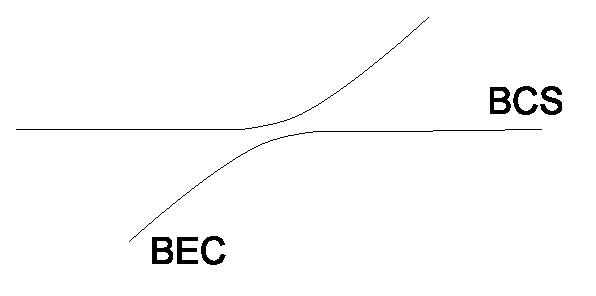
\includegraphics[width=.50\textwidth]{image/levelCross}
	\caption{Level Crossing in Feshbach Resonance \label{fig:levelcross}}	
\end{figure}
 Actually at this point, $a_s$ is no longer important physically as most particles are in close-channel and open-channel component is mostly due to inter-channel coupling from close-channel instead. This is expected to last until the detuning is so large that the transition between two-channels are slow enought that we no longer need to take the coupling into consideration, i.e it is no longer a two-channel problem and back to only single open-channel problem (samples are prepared in open-channel and there are no any significant conversion within the time-frame of experiments).  

\subsection{$\Delta$ and $\alpha$ in gap/number equations}
However, we still have the problem with $\Delta$ and $\alpha$.  
\begin{equation}\label{eq:20101011:delta}
\Delta_{\vk}=U_{\vk\vk'}F_{\vk'}+Y_{\vk\vk'}G_{\vk'}\approx\alpha{Y_{\vk\vk'}\phi^{0}_{\vk'}}
\end{equation}
They are related by \eef{eq:20101011:delta}, it is clear that the first term $U_{\vk\vk'}F_{\vk'}$ can be neglected when close-channel domintes, and $\Delta$ is propotional to $\alpha$ and gets satuated toward the BEC extreme (here the extreme means the close-channel dominated molecules).  The relation is relatively complicated when open-channel is not small. In the two-body, around universality, open-channel weight goes to infinity and clearly domintes, but many-body seems put a natual upper-bound on it . It is possible that $F_{\vk'}$ is always finite and  this term ($U_{\vk\vk'}F_{\vk'}$ ) might never be important.  

If we keep only one of $\Delta$ and $\alpha$, we need to make an assumption that $U_{\vk\vk'}F_{\vk'}$ term is always dominated and we still need to have paramiter $Y_{\vk\vk'}\phi^{0}_{\vk'}$ that relates these two quantities. 
\begin{equation}\label{eq:20101011:deltaAlpha}\Delta^{2}\approx\alpha^{2}(\Delta^{2}|_{\text{very BEC end}})
\end{equation}
Here we can see that $\Delta$ saturates in BEC end where close-channel dominates.   On the other hand, we need one extra equation (likely \eef{eq:20101011:delta}) to keep both of them, which requires the detail information of $Y_{\vk\vk'}$ as well as $U_{\vk\vk'}$.  (Not clear????)